\section{Evaluation}
\label{sec:eval}
To perform the evaluation of the solver we used table of real Java classes of size 40960.
And we evaluate the following 9 queries, each of which corresponds to a group of 4 columns in the Fig.~\ref{fig:eval-diagram}.
\begin{itemize}
    \item The first 4 queries are 1, 2 and 3 upper bounds for standard collection classes and interfaces \java{List}, \java{AbstractCollection} and \java{RandomAccess}. Note, the 2nd and the 3rd queries are the same 2 upper bounds but with opposite order.
    \item The next 3 queries are 1, 2 and 3 lower bound for concrete collection classes \java{AttributeList}, \java{PersistentVector} and \java{ImmutableSortedSet}.
    \item The last 2 queries consist of one upper bound and one lower bound. These bounds the same for both queries but with opposite order.
\end{itemize}

\begin{figure}[h]
  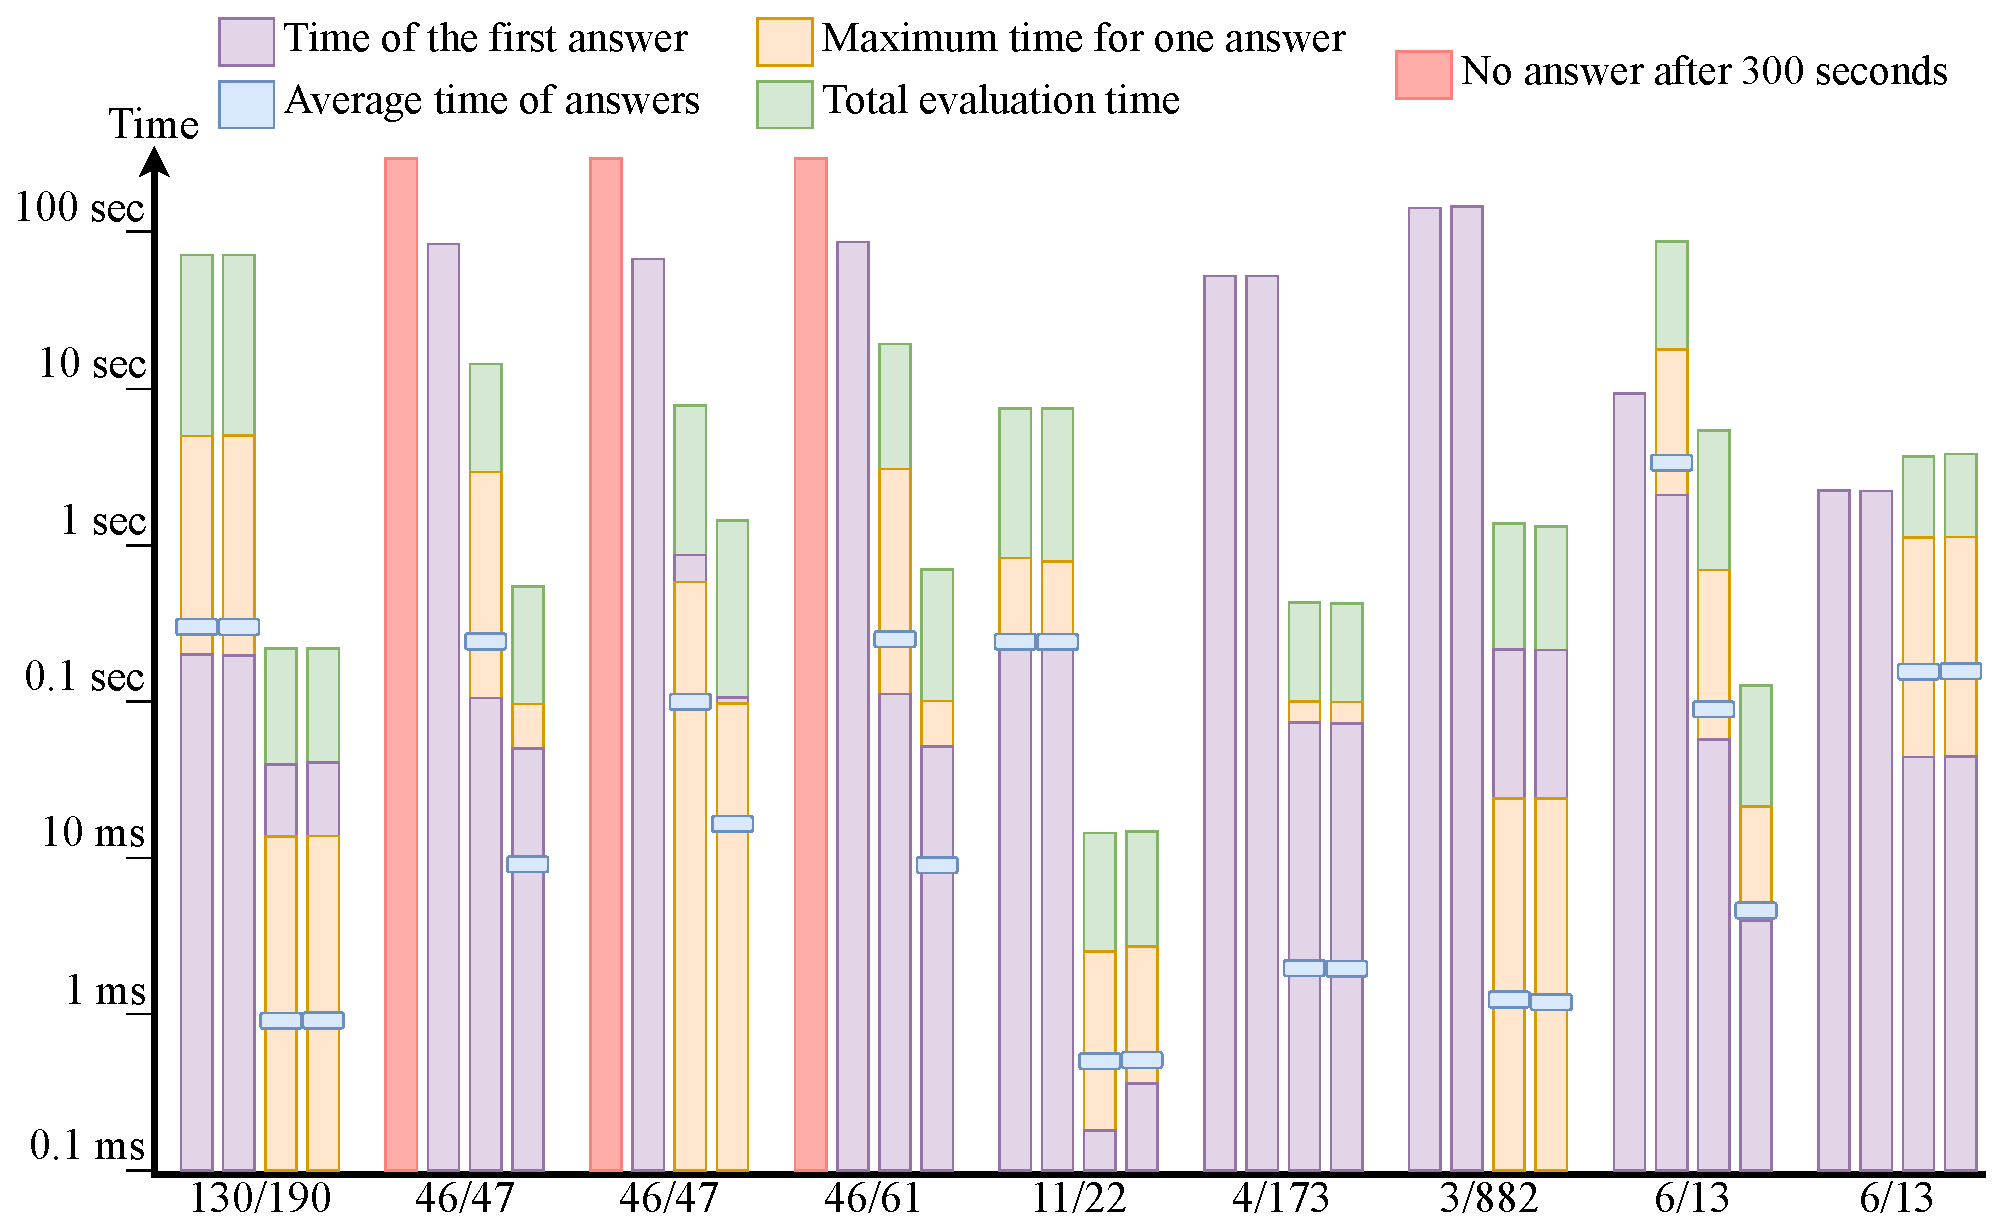
\includegraphics[width=1\textwidth]{eval_diagram.eps}
  \caption{Evaluation results of 9 queries to the table of real Java classes of size 40960 for 4 versions of the solver.}
  \label{fig:eval-diagram}
\end{figure}

Each query was evaluated for 4 solver versions: without optimizations (the first column for each query), with dynamic transitive closure (the second column), with dynamic class table specialization (the third column) and with both optimizations (the fourth column). In all these versions, the capture conversion is disabled.
For each query we evaluated 2 quantitative measures: answers amount (numerator under column group), unique answers amount (denominator). Also we evaluated 4 time measures: time of the first answer (this time includes the time spent on the pre-calculations required to dynamic table specialization), maximum time for one answer (not include the first answer time), average time of all answers and total evaluation time. We also limited the evaluation time to 300 seconds. And in several cases, we either received only a part of the answers (in this case, only the time for calculating the first answer is indicated), or we did not receive a single answer (in this case, the red column is shown in the figure). These measurements are presented on a logarithmic scale.

As we can see from the results presented in the picture, dynamic transitive closure improves the result by an order of magnitude in some cases (if there is an upper bound among the second and subsequent bounds), dynamic specialization of the table always improves the result by an order of magnitude, but the best performance is achieved when using both optimizations. It is also noteworthy that for queries with the same bounds but different orders (3rd, 4th and 8th, 9th), the time dimensions are different. Therefore, the efficiency of the solver depends on the order of the boundaries. Finally, It can be noted that when calculating the lower bounds, we get a large number of duplicate answers.

We can conclude that the optimized version of the solver with disabled capture conversion shows promising performance results, but the problems of the influence of the order of bounds and the presence of duplicates require further research.

\begin{comment}

%\begin{figure}[h]
%  \makebox[\textwidth][c]{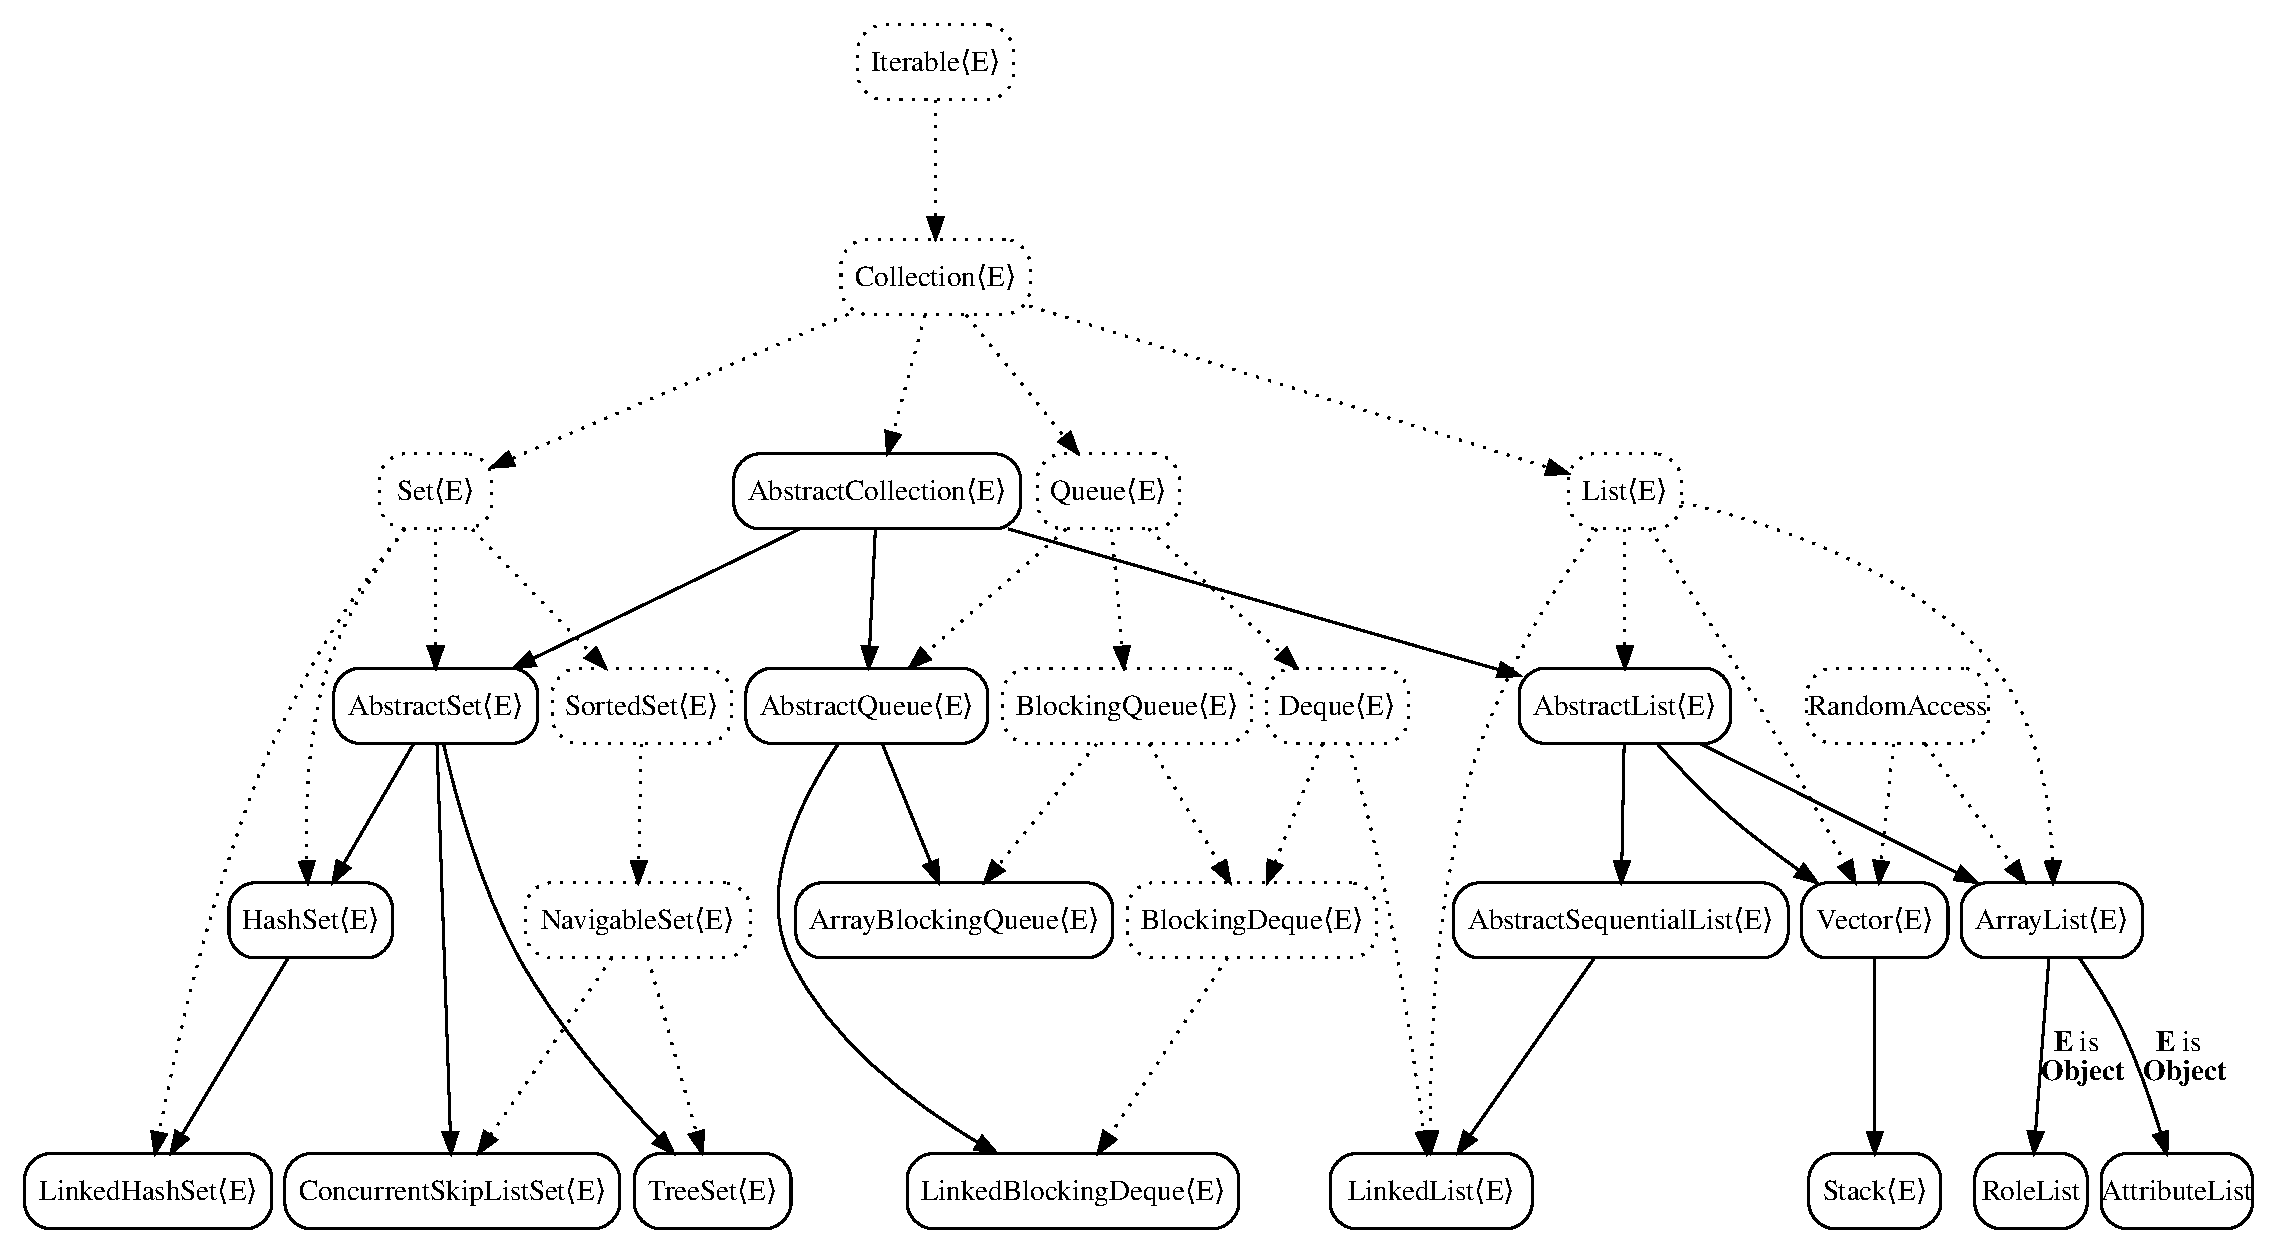
\includegraphics[width=1.3\textwidth]{class_graph.eps}}
%  \caption{Evaluation class table: a subset of \textsc{Java} collection classes}
%  \label{fig:class-graph}
%\end{figure}

    On pic.~\ref{fig:class-graph} class \textbf{AbstractCollection} extends class \textbf{Object}. Also classes \textbf{ArrayList}, \textbf{Vector}, \textbf{LinkedList}, \textbf{HashSet}, \textbf{TreeSet}, \textbf{ConcurrentSkipListSet} and \textbf{LinkedHashSet} implements interfaces \textbf{Cloneable} and \textbf{Serializable}. Classes \textbf{BlockingQueue} and \textbf{LinkedBlockingDeque} implements interface \textbf{Serializable} only.

To perform the evaluation of the solver we came up with we prepared a sample class table using a subset of standard \textsc{Java} collection classes and interfaces. The
inheritance graph for this subset is shown in Fig.~\ref{fig:class-graph}; the nodes with solid border correspond to classes, with dashed border~--- to interfaces.

Our first attempt discovered the fact that the solver was unsound~--- it established the subtyping relation for two arbitrary types. This finding constitutes a drastic
contradiction with the theory which predicts that the solver has to be correct by construction. The careful analysis, however, discovered that functional
vefifier was unsound as well! The reason was very simple: let us have two arbitrary types $A$ and $B$. To establish, for example, that $A \precprec B$, take a
type variable $\alpha^B_A$ with upper bound $B$ and lower bound $A$. Then, by definition

\[
A\precprec \alpha^B_A \wedge \alpha^B_A\precprec B \Rightarrow A\precprec B
\]

In the JLS there were no explicit requirement for lower/upper bounds of type variables to respect the subtyping relation, thus this requirement was not
encoded in the verifier.

Another finding of the evaluation was that, contrary to the expectation, the direct supertyping relation is actually reflexive (in full accordance with the JLS).

\begin{figure}[h]
    \begin{tabular}{c|c|c|c|c}
        \multirow{2}{*}{Test} & \multicolumn{2}{c|}{JGS} & \multicolumn{2}{c}{Simplified JGS} \\
        \cline{2-5}
         & Time & Answers & Time & Answers \\
         \hline
         
         ? $\precprec$ AbstractList\textlangle Object\textrangle 
         & 1.152
         & 8 / 8
         & 0.238
         & 8 / 8
         \\ \hline
         RoleList $\precprec$ ? 
         & 0.472
         & 38 / 21
         & 0.332
         & 22 / 11
         \\ \hline
         ? $\precprec$ Iterable\textlangle Object\textrangle 
         & $>$300
         & -
         & 1.912
         & 58 / 26
         \\ \hline
         ? $\precprec$ RandomAccess $\land$
         & $>$300
         & -
         & 1.326
         & 8 / 5
         \\
         ? $\precprec$ AbstractCollection\textlangle Object\textrangle 
         &&&&\\ \hline
        LinkedList\textlangle Object\textrangle $\,\precprec$ ? $\land$
        & 24.278
        & 95 / 10
        & 3.620
        & 69 / 6
        \\
        TreeSet\textlangle Object\textrangle $\,\precprec$ ?
        &&&&
    \end{tabular}
    \caption{The results of evaluation for some queries}
    \label{fig:eva}
\end{figure}

After we added explicit subtyping constraint for the bounds of type variables, we could, indeed, obtain all correct subtyping results
    for queries we took for evaluation. The results are shown in Fig.~\ref{fig:eva}.

    We encountered a few other issues. First, in the presence of capture conversion the solver works very slow and can not always
    provide answers in a reasonable time even for very simple queries (see column JGS). However, capture conversion makes the
    solver return wildcard types which are not instantiable (can not be used as types of concrete data values). In the
    scenario of usage we are aimed at such types are meaningless. Thus we evaluated a simplified version of the solver with
    capture conversion switched off (see Simplified JGS column).    
    
    Another issue is that the solver tends to return duplicating answers. In the columns ``Answers'' the numerator gives the number of
    returned answers while denominator~--- the total number of correct pairwise distinct solutions.

    We can conclude that, first, our approach discovers the incompleteness in specifications and, second, that the simplified version
    with capture conversion switched off shows a promising performance results.

\end{comment}



